% chapters/05_ergebnisse.tex

\chapter{Ergebnisse}
\label{chap:ergebnisse}

Laufnummern verweisen auf \doc{docs/ergebnisse/diagnose-chronik.md}.

\section{Training und Checkpoint-Wahl}
\label{sec:erg-training}
\label{sec:trainingsverlauf}
\label{sec:lernkurven}
\label{sec:lauf3}

\begin{table}[htb]
  \centering
  \begin{tabularx}{\linewidth}{lXrr}
    \toprule
    Lauf & Konfiguration & Schritte & Dauer \\
    \midrule
    1 & N1.6, 1$\times$A100, Bild-Encoder eingefroren, alle Episoden, kein Split & 175\,000 & 21,4~h \\
    2 & N1.6, 4$\times$A100, Bild-Encoder mittrainiert, kein Split & 44\,000 & 8,4~h \\
    3 & wie 2, dazu Split 240/61 und Farb-Augmentierung (\enquote{vision-v2}) & 44\,000 & 12,5~h \\
    4 & N1.7, sonst wie 3, State-Dropout 0,2 & 44\,000 & 7~h~53~min \\
    \bottomrule
  \end{tabularx}
  \caption{Trainingsläufe (Batch 8 bzw.\ 32, Lernrate \num{1e-4}; Details:
    \cref{tab:hparams}). Ob Lauf~2 schon mit Augmentierung lief, ist nicht sicher belegt.}
  \label{tab:laeufe}
\end{table}

Alle Läufe konvergieren ohne Spitzen (\cref{fig:lernkurven}; Läufe 1--3:
\cref{fig:loss-curve}). Der Trainings-Loss trennt die Konfigurationen nicht, zwischen N1.6 und
N1.7 ist seine Höhe nicht vergleichbar (anderer Aktionskopf, State-Dropout). Die
Checkpoint-Wahl beruht deshalb auf der Open-Loop-\ac{mse} auf 20 Testepisoden à 750 Schritte:
Alle 16 Schritte sagt das Modell aus echten Bildern und echtem Zustand einen Aktionsblock
voraus, der vollständig mit den aufgezeichneten Aktionen verglichen wird; gemittelt wird
unnormiert (rad²) über alle 28 Dimensionen und Schritte, dann über die Episoden.
Checkpoints werden mit dem gepaarten t-Test über die 20 Episoden verglichen (zweiseitig).

\begin{figure}[htb]
  \centering
  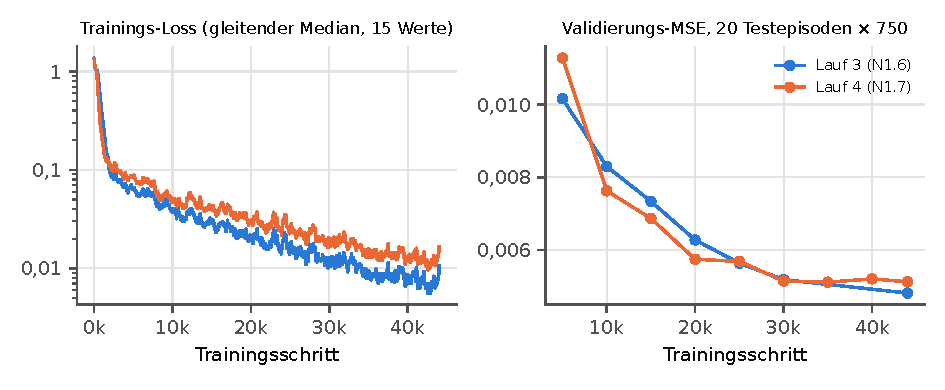
\includegraphics[width=\linewidth]{figures/plots/lernkurven_lauf3_lauf4.pdf}
  \caption{Lauf~3 (N1.6) und Lauf~4 (N1.7). Links Trainings-Loss (Offline-Logs auf KISSKI, in \ac{wandb} synchronisiert), rechts Validierungs-\ac{mse} je Checkpoint
    (\doc{docs/ergebnisse/lauf4-n17-vergleich.md}, §5).}
  \label{fig:lernkurven}
  \label{tab:val-mse}
\end{figure}

\begin{itemize}
  \item Bei N1.6 fällt die \ac{mse} bis 44\,000 monoton auf 0,00482; 44\,000 ist signifikant
    besser als 30\,000 ($t = 2{,}15$, $p = 0{,}045$). Eine frühere Auswertung auf 6 Episoden à 300 Schritte
    hatte ein Optimum bei 30\,000 gezeigt; das war ein Effekt der kurzen Auswertung.
  \item N1.7 ist am besten bei 35\,000 (0,00512); gegen N1.6 @44000 ist der Unterschied nicht
    signifikant ($+6\,\%$, $t = 1{,}20$, $p = 0{,}25$). N1.7 lernt früher (signifikant besser bei 10\,000 und
    20\,000) und trainiert 1,6-mal so schnell. State-Dropout und Normierung weichen ab; der
    Vergleich ist einer von Modell und Rezept. Gemessen wird N1.7 trotzdem @44000: Gegen
    @35000 ist der Unterschied nicht messbar ($t = 0{,}05$, $p = 0{,}96$), und alle Modelle haben so dieselbe
    Schrittzahl.
\end{itemize}

Gute Open-Loop-Werte auf echten Bildern sagen wenig über den Closed Loop in der Simulation
(\cref{sec:erg-closed-loop}).

\section{Closed Loop ohne Co-Training}
\label{sec:erg-closed-loop}
\label{sec:closed-loop-ergebnis}
\label{sec:realperformance}

Die Inferenz-Kette (Checkpoint laden, Server, \ac{zmq}, Zuordnung von Beobachtung und Aktion)
ist extern geprüft: Das nicht nachtrainierte Basismodell N1.6 erreicht damit auf der
Referenzaufgabe RoboCasa GR-1 Tabletop~\cite{robocasa2024} 47,7\,\% gegen veröffentlichte
47,8\,\% (12 von 24 Teilaufgaben, je 100 Episoden). Das Scheitern im Closed Loop liegt deshalb
nicht am Modellaufruf; die eigene Isaac-Lab-Szene prüft dieser Test nicht.

Kein Modell hebt in der Simulation einen Würfel frei an
(\cref{tab:cl-ohne}). N1.6 fährt die Würfel meist an und berührt sie (17/20), N1.7 seltener
(7/20); keine Policy schließt die Hand um einen Würfel.

\begin{table}[htb]
  \centering
  \begin{tabular}{llrrrr}
    \toprule
    Lauf & Modell & Episoden & \texttt{reached} & \texttt{touched} & \texttt{lifted\_clear} \\
    \midrule
    34 & N1.6 vision-v2 @30000, alte Szene\textsuperscript{a} & 10 & 9 & 10 & n.\,e.\textsuperscript{b} \\
    55 & N1.7 @44000 & 10 & 9 & 6 & n.\,e.\textsuperscript{b} \\
    81 & N1.7 @44000, Szene Lauf 70 & 20 & 7 & 7 & 0 \\
    82 & N1.6 vision-v2 @44000, Szene Lauf 70 & 20 & 16 & 17 & 0 \\
    \bottomrule
  \end{tabular}
  \caption{Closed Loop ohne Co-Training. \textsuperscript{a}Vor der Korrektur vom 24.08.2026:
    Fingergelenke falsch gespiegelt, Becken 0,85~m statt 0,764~m (\cref{sec:projektverlauf-fehler}).
    \textsuperscript{b}Nicht erfasst: \texttt{lifted\_clear} gibt es erst seit 13.10.2026; das schwächere Kriterium \texttt{lifted} lag bei 0/10.
    95-\%-Intervall für 0/20: 0--17\,\%.}
  \label{tab:cl-ohne}
\end{table}

\section{Blocker 1: Lage der Würfel relativ zur Hand}
\label{sec:erg-registrierung}
\label{sec:geometrie}
\label{sec:wuerfellage}

Um Modell und Simulation zu trennen, spielt ein Demo-Replay (engl.\ \emph{oracle replay}) die
aufgezeichneten Aktionen des menschlichen Bedieners für die jeweilige Testepisode ohne Modell und
ohne Rückkopplung ab. Gelingt die Aufgabe selbst so nicht, liegt der Fehler in der Szene; das
Replay ist damit die praktische Obergrenze, an der sich jede Policy messen lässt. Auf den aus Bildern bestimmten Würfellagen hebt es \texttt{lifted\_clear} 1/16
(95-\%-Intervall 0,2--30\,\%, Lauf~57): Die Hand erreicht und schließt, schiebt oder kippt den
Würfel aber. Die Griffstellen der echten Hand liegen 1--7~cm neben der Würfellage aus dem
Bild, seitlich spiegelbildlich je Hand (Lauf~59). Die Würfelgröße ist nicht die Ursache
(Lauf~58).

\begin{figure}[htb]
  \centering
  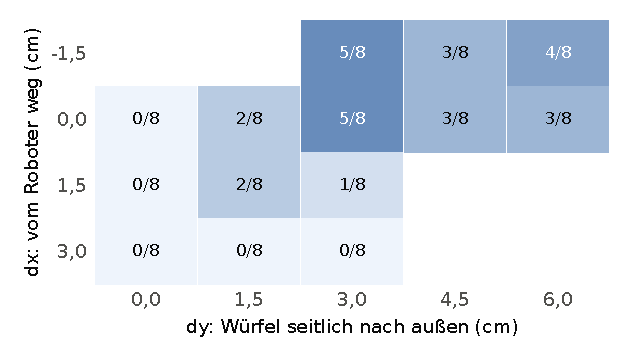
\includegraphics[width=0.62\linewidth]{figures/plots/orakel_versatz_lauf62.pdf}
  \caption{Demo-Replay mit verschobenen Würfeln: \texttt{lifted\_clear} von 8 Episoden je
    Verschiebung (Lauf~62). Leere Felder wurden nicht gemessen.}
  \label{fig:orakel-sweep}
\end{figure}

Ein Raster über die Verschiebung (\cref{fig:orakel-sweep}) zeigt: Ohne seitliche Korrektur
hebt das Replay in 0 von 24 Episoden, mit 3--6~cm nach außen (bei $dx \le 0$) in 23 von 48. Bei $dx = 0$ trennt
sich $dy = 3$~cm (5/8) von $dy = 0$ (0/8) mit $p \approx 0{,}03$ (exakter Fisher-Test). Die
Würfel liegen in der Simulation relativ zur Hand also je Seite rund 3~cm zu weit innen. Mit
dieser Korrektur hebt das Replay auf 20 Testlagen in 6 Fällen frei an (30\,\%,
95-\%-Intervall 12--54\,\%, Lauf~69).

Die Ursache ist offen. Kein einzelner Gelenk-Nullpunkt erklärt den Versatz, eine
mitwandernde Kopfkamera ist widerlegt (Lauf~63). Alle Closed-Loop-Messungen ab Lauf~81
verwenden die empirische Korrektur (\texttt{layout\_heldout\_dy3.json}).

\section{Blocker 2: Visueller Domain-Gap}
\label{sec:erg-domain-gap}
\label{sec:domain-gap-ergebnis}

\begin{figure}[htb]
  \centering
  \begin{subfigure}[t]{0.48\linewidth}
    \centering
    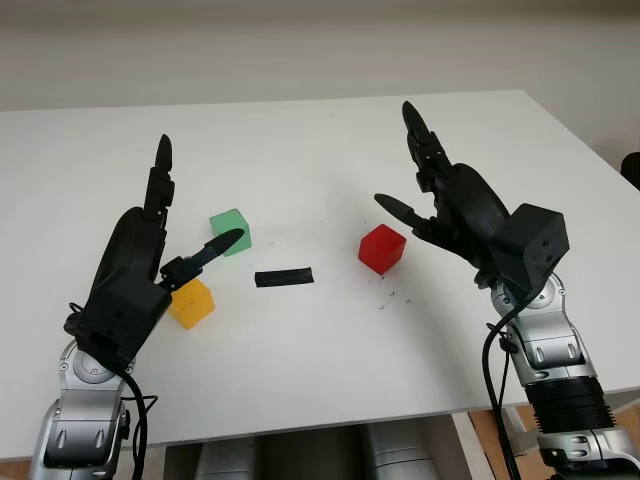
\includegraphics[width=\linewidth]{figures/sim/real_cam_left_high.png}
    \caption{Datensatz}
  \end{subfigure}\hfill
  \begin{subfigure}[t]{0.48\linewidth}
    \centering
    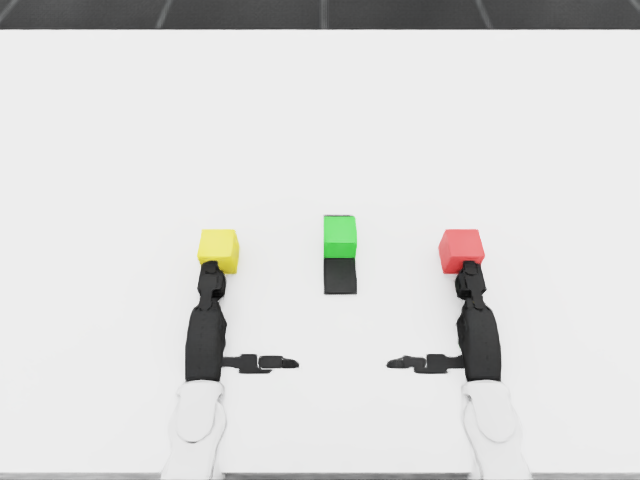
\includegraphics[width=\linewidth]{figures/sim/sim_scene70_cam_left_high.png}
    \caption{Simulation, Szene aus Lauf 70}
  \end{subfigure}
  \caption{Linke Kopfkamera. Die Geometrie stimmt auf 10--20 Pixel; Tisch, Licht, Material
    und Hintergrund unterscheiden sich (Lauf~67).}
  \label{fig:domain-gap}
\end{figure}

Die Wirkung der Bilder lässt sich ohne Regelkreis messen: Die Policy sagt teacher-forced
Aktionen für denselben Zustand einmal auf echten und einmal auf gerenderten Bildern derselben
Episode vorher (\cref{tab:domain-gap}).

\begin{table}[htb]
  \centering
  \begin{tabular}{lrrrr}
    \toprule
    Bilder & \multicolumn{2}{c}{N1.6} & \multicolumn{2}{c}{N1.7} \\
    \midrule
    alle echt & 0,0020 & & 0,0017 & \\
    nur Kopfkameras simuliert & 0,0086 & ($\times$4) & 0,0073 & ($\times$4) \\
    nur Handgelenkkameras simuliert & 0,0090 & ($\times$4) & 0,0340 & ($\times$20) \\
    alle simuliert & 0,0269 & ($\times$13) & 0,0606 & ($\times$36) \\
    \bottomrule
  \end{tabular}
  \caption{\ac{mse} der Hand-Aktionen (Median über 8 Trainingsepisoden; Läufe 66 und 71).}
  \label{tab:domain-gap}
\end{table}

Der Fehler steigt in dieselbe Größenordnung wie mit schwarzen Bildern (Lauf~65): Für die
Policy tragen die Sim-Bilder ungefähr so viel verwertbare Information wie kein Bild. N1.6
leidet unter beiden Kameragruppen, N1.7 vor allem unter den Handgelenkkameras. Die Szene wurde
daraufhin ans Echtbild angeglichen (breiterer Tisch, Handgelenkkamera näher an der echten
Pose, 85° Öffnungswinkel; Lauf~70). Das senkt den Fehler um 40\,\% (N1.6) bzw.\ 18\,\%
(N1.7); er bleibt aber das 8- bzw.\ 29-Fache des Echtbilds. Grobe Szenenmerkmale erklären also
nur einen kleinen Teil.

\section{Co-Training mit gerenderten Bildern}
\label{sec:erg-cotrain}
\label{sec:cotrain}

\paragraph{Daten und Läufe.} Co-Training auf echten und simulierten Daten ist eine übliche Gegenmaßnahme zum Domain-Gap~\cite{cotrain2025}, neben \ac{dr}~\cite{tobin2017domain} und der Angleichung der Simulationsoptik~\cite{simpler2024}. Die echten Aktionen von 187 der 240 Trainingsepisoden wurden in der
Szene aus Lauf~70 abgespielt und mit allen vier Kameras gerendert (29\,890 Frames), einmal mit
5-cm- und einmal mit 4-cm-Würfeln (Lauf~72). Nicht gerendert wurden die vier Episoden des
Prüfsets, drei Episoden mit unsicherer Würfellage, eine im Rendern hängende Episode und 45
Episoden mit zu kurzem Fenster vor dem Griff. Gemischt wird mit Anteil 0,15 gerendert, knapp über
dem Frame-Verhältnis 0,115. Vier Läufe auf KISSKI (Läufe 73--76, je 44\,000 Schritte): N1.6 und
N1.7, jeweils mit beiden Würfelgrößen (\cref{tab:cotrain-namen}). Die Validierungs-\ac{mse} auf
echten Testepisoden liegt im selben Protokoll (20 Episoden à 750 Schritte) 3--9\,\% über
Lauf~3.

\begin{table}[htb]
  \centering
  \begin{tabular}{lll}
    \toprule
    & Würfel 5~cm & Würfel 4~cm \\
    \midrule
    N1.6 & B (Lauf 73) & C (Lauf 74) \\
    N1.7 & A (Lauf 75) & D (Lauf 76) \\
    \bottomrule
  \end{tabular}
  \caption{Bezeichnung der Co-Training-Läufe.}
  \label{tab:cotrain-namen}
\end{table}

\paragraph{Visuelles Gate.} Alle co-trainierten Modelle senken den Hand-Fehler auf den
Sim-Prüfbildern deutlich (\cref{fig:gate}): N1.6 auf 47--49\,\% des Ausgangswerts, N1.7 auf
18--30\,\%. Auf Echtbildern bleibt N1.7 gleich (0,0024--0,0027 gegen 0,0026), N1.6 wird um
50--60\,\% schlechter (0,0014 $\to$ 0,0021--0,0022). Das Gate trennt aber nicht zuverlässig
\enquote{co-trainiert} von \enquote{nicht co-trainiert}: Auch die alten N1.6-Modelle (Lauf~1,
vision-v1) unterbieten die 80-\%-Schwelle (Lauf~87). Die Gate-Werte sind nicht direkt mit
\cref{tab:domain-gap} vergleichbar: Das Gate nutzt 4 Episoden à 600 Schritte mit festen Seeds,
die Tabelle 8 Episoden ohne Seed.

\begin{figure}[htb]
  \centering
  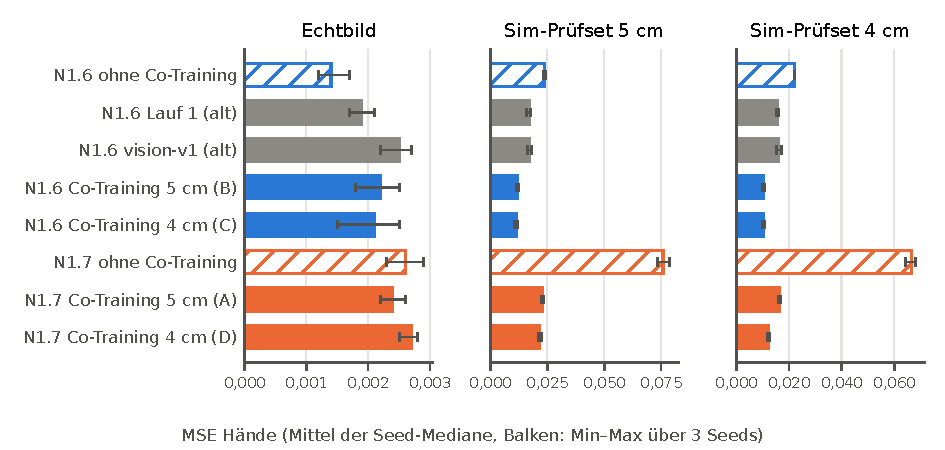
\includegraphics[width=\linewidth]{figures/plots/gate_mse_haende.pdf}
  \caption{Visuelles Gate: \ac{mse} der Hand-Aktionen auf Echtbildern und gerenderten
    Prüfbildern; schraffiert die Ausgangswerte ohne Co-Training. Daten aus den Läufen 80, 83, 86, 87 und 92.}
  \label{fig:gate}
\end{figure}

\paragraph{Closed Loop.} Mit Co-Training erreichen und berühren die Policies die Würfel in
fast jeder Episode (\cref{fig:closed-loop}). Echte Griffe, im Video bestätigt, gibt es nur bei
N1.6: C hebt auf allen 60 Testlagen in 2 Episoden frei an (\texttt{lifted\_clear} 2/60 =
3\,\%, 95-\%-Intervall 0,4--11,5\,\%, Läufe 88 und 97), B in 1 von 20 (Lauf~84). Beide N1.7-Modelle heben nicht frei an
(0/20, Läufe 89 und 93); die 6 \texttt{lifted} von A sind Schieben und Kippen. Gestapelt wird
in keiner Episode. Gegen 0/20 ohne Co-Training (Lauf~82) ist 2/60 statistisch nicht zu
trennen (exakter Fisher-Test, einseitig, $p \approx 0{,}56$).

\begin{figure}[htb]
  \centering
  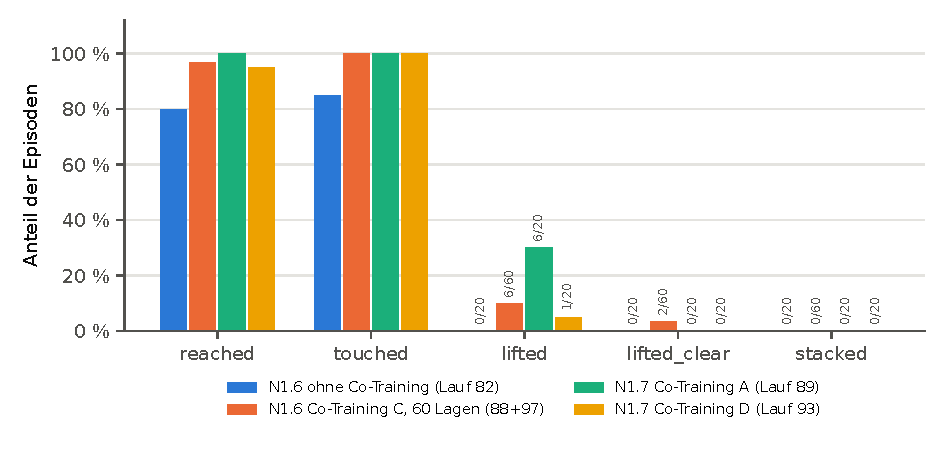
\includegraphics[width=\linewidth]{figures/plots/closed_loop_stufen.pdf}
  \caption{Closed Loop, 120~s je Episode, Testlagen mit 3-cm-Korrektur. \texttt{lifted} ohne
    Artefakte (weggeschleuderte Würfel).}
  \label{fig:closed-loop}
\end{figure}

\begin{figure}[htb]
  \centering
  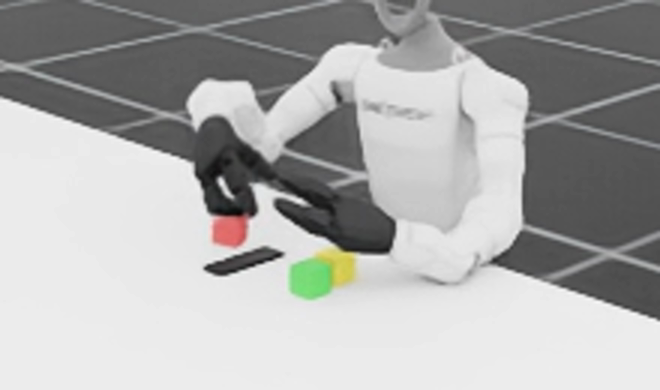
\includegraphics[width=0.7\linewidth]{figures/sim/griff_lauf88_ep05_80s_ausschnitt.png}
  \caption{Erster Griff einer Policy: Modell C, Lauf~88, Episode~5, $t = 80$~s. Die linke
    Hand hält den roten Würfel in der Luft.}
  \label{fig:griff}
\end{figure}

\paragraph{Vorregistriertes Gate.} Vor dem Co-Training war festgelegt: Liegt die Fingerspanne
im Closed Loop (10 Episoden à 40~s) deutlich über 0,577~rad = 27,6\,\% (Lauf~34), trägt der
Weg. Zwei Einschränkungen: \enquote{deutlich} war nicht als Zahl festgelegt, und Lauf~34 stammt
aus der Szene vor der Korrektur vom 24.08. Aussagekräftiger ist deshalb der Vergleich in der
heutigen Szene. Modell C erreicht 1,53~rad = 73\,\% der Demonstration (Lauf~96, \cref{fig:spanne}).
Gegen dasselbe Rezept ohne Renderdaten in der heutigen Szene (vision-v2, 0,52~rad) ist das
$p = 5\cdot10^{-6}$, gegen die alte Referenz $p = 0{,}001$ (exakter Rangtest, einseitig). Gegen das alte Lauf-1-Modell (1,21~rad) ist
es nur eine Tendenz ($p = 0{,}07$): Weit öffnen können auch Modelle ohne Co-Training. Belastbar
sind damit das veränderte Verhalten (\texttt{touched} 60/60 gegen 17/20, gleichmäßig weite
Spanne), nicht die Griffrate.

\begin{figure}[htb]
  \centering
  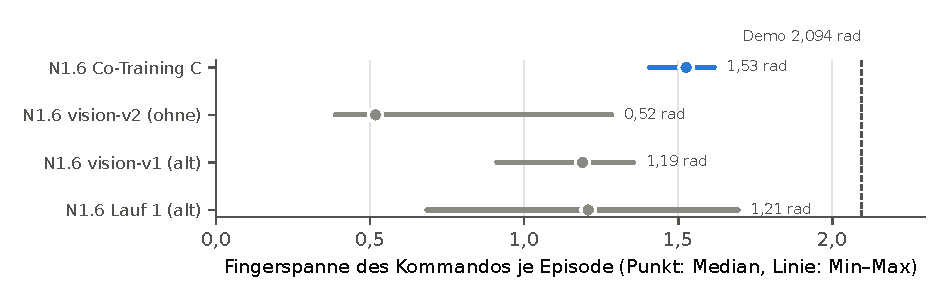
\includegraphics[width=\linewidth]{figures/plots/fingerspanne_lauf96.pdf}
  \caption{Fingerspanne im Closed Loop, 10 Episoden à 40~s (Lauf~96).}
  \label{fig:spanne}
\end{figure}

\section{N1.7 gegen N1.6}
\label{sec:erg-n17}
\label{sec:n17}

N1.7 ist im Open Loop auf echten Bildern gleichauf mit N1.6 und schneller trainiert. Auf
Sim-Bildern ist es ohne Co-Training deutlich schlechter ($\times$36 gegen $\times$13), mit
Co-Training erreicht es auf den Prüfbildern etwa das Niveau des nicht co-trainierten N1.6.
Im Closed Loop greift kein N1.7-Modell. Für die Simulation ist N1.6 mit Co-Training der beste
Kandidat (\texttt{luca-mue/groot-g1dex3-cotrain-v3-cube4-ckpt44000}).
